\documentclass{beamer}

%------------------------------------
%------------Libraries---------------
%------------------------------------

\usepackage[brazil]{babel}
\usepackage[utf8]{inputenc}
\usepackage{xpatch}
\usepackage{ragged2e}
\usepackage{xcolor}
\usepackage{url, hyperref}
\usepackage[portuguese,ruled,vlined]{algorithm2e}

\usepackage{amsmath, amsthm, amssymb, amsfonts}
\usepackage{subfig}

\usepackage{natbib}

%------------------------------------
%----------Configurations------------
%------------------------------------

\usetheme{Madrid}
\usecolortheme{default}
\useinnertheme{circles}

\definecolor{FirstColor}{rgb}{0.0157,0.2392,0.4902}
\definecolor{SecondColor}{rgb}{0.0157, 0.549, 0.8}

\setbeamertemplate{itemize items}[triangle]

\setbeamercolor*{palette primary}{bg=FirstColor, fg=white}
\setbeamercolor*{palette secondary}{bg=SecondColor, fg=white}
\setbeamercolor*{palette tertiary}{bg=white, fg=FirstColor}
\setbeamercolor*{palette quaternary}{bg=FirstColor,fg=white}
\setbeamercolor{structure}{fg=FirstColor}
\setbeamercolor{section in toc}{fg=FirstColor}

\hypersetup{colorlinks=true,citecolor=blue, urlcolor = cyan, linkcolor=blue}

\apptocmd{\frame}{}{\justifying}{}

%---------------------------------------------------
%------------------Itemize--------------------------
%---------------------------------------------------

\makeatletter
\newcommand{\my@beamer@setsep}{%
\ifnum\@itemdepth=1\relax
     \setlength\itemsep{\my@beamer@itemsepi}% separation for first level
   \else
     \ifnum\@itemdepth=2\relax
       \setlength\itemsep{\my@beamer@itemsepii}% separation for second level
     \else
       \ifnum\@itemdepth=3\relax
         \setlength\itemsep{\my@beamer@itemsepiii}% separation for third level
   \fi\fi\fi}
\newlength{\my@beamer@itemsepi}\setlength{\my@beamer@itemsepi}{3ex}
\newlength{\my@beamer@itemsepii}\setlength{\my@beamer@itemsepii}{1.5ex}
\newlength{\my@beamer@itemsepiii}\setlength{\my@beamer@itemsepiii}{1.5ex}
\newcommand\setlistsep[3]{%
    \setlength{\my@beamer@itemsepi}{#1}%
    \setlength{\my@beamer@itemsepii}{#2}%
    \setlength{\my@beamer@itemsepiii}{#3}%
}
\xpatchcmd{\itemize}
  {\def\makelabel}
  {\my@beamer@setsep\def\makelabel}
 {}
 {}

\xpatchcmd{\beamer@enum@}
  {\def\makelabel}
  {\my@beamer@setsep\def\makelabel}
 {}
 {}
\makeatother

%---------------------------------------------------
%-----------------Definitions-----------------------
%---------------------------------------------------

\newcommand{\Space}{\vspace{3ex}}
\newcommand{\R}{\mathbb{R}}
\newcommand{\onevec}{\boldsymbol{e}}
\newcommand{\ev}{\mathbb{E}}
\newcommand{\var}{\operatorname{Var}}
\newcommand{\cor}{\operatorname{Cor}}
\newtheorem{proposition}[theorem]{Proposição}

%---------------------------------------------------
%----------------Front page-------------------------
%---------------------------------------------------

\title[Bootstrap]
{Bootstrap \\ \small Uma leitura de Efron e Tibshirani (1986)}
%\subtitle{}
\pdfstringdefDisableCommands{%
  \def\\{}%
  \def\texttt#1{<#1>}%
}
\author[Lucas]
{      
    Lucas Machado Moschen
}
\institute[]
{
  Escola de Matemática Aplicada \\
  Fundação Getulio Vargas
}
\date[\today]
{\today}

\titlegraphic{
    \vspace*{0.3cm}
    \hspace*{9.5cm}
    
\includegraphics[width=.2\textwidth]{logo-emap.png}
}
%--------------------------------------------------

%---------------------------------------------------
%---------------- Document -------------------------
%---------------------------------------------------

\begin{document}

\frame{\titlepage}

\section{Introdução}

\begin{frame}{Bootstrap}
    \begin{itemize}
        \item Técnica desenvolvida com objetivo de medir a acurácia de
        estimadores; 

        \bigskip

        \item É mais utilizado na abordagem frequentista, mas pode ser
        interpretado na Bayesiana \cite[]{rubin1981bayesian};

        \bigskip

        \item A ideia geral é gerar novos pontos a partir dos iniciais e
        proceder a estimação em cada conjunto de dados, gerando uma
        distribuição para o estimador.
    \end{itemize}
\end{frame}

\begin{frame}{Bootstrap}

    A construção de \cite{Efron1986} supõe que observamos $\boldsymbol{x} = (x_1, x_2,
    \dots, x_n)$ de 
    $$
    \boldsymbol{X} = (X_1, X_2, \dots, X_n), X_i \overset{iid}{\sim} F, 
    $$
    em que $F$ é distribuição desconhecida. Podemos relaxar para dados dependentes.
    \cite[]{lahiri1999theoretical}.
    
    \bigskip\pause
    
    Sejam $R(\boldsymbol{X}, F)$ a variável de interesse como a estatística
    $\hat{\theta}(\boldsymbol{X})$, e $\hat{F}$ a distribuição empírica de
    $\boldsymbol{x}$.
    
    \bigskip\pause
    
    Vamos utilizar estimadores de Monte Carlo para aproximar aspectos de da
    distribuição de $R$, como $\ev_{\hat{F}}[R]$.

\end{frame}

\begin{frame}{Erro padrão}

    Um exemplo usual é o erro padrão
    $$\sigma_F = \left(\var_F(\hat{\theta}(\boldsymbol{X}))\right)^{1/2}$$
    de uma estatística $\hat{\theta}(\boldsymbol{X})$ 
    que pode ser aproximada por 
    $$
    \hat{\sigma}_{\hat{F}} = \left(\var(\hat{\theta}_
    {\hat{F}}(\boldsymbol{x}))\right)^{1/2}
    $$
    que é o desvio padrão com $F = \hat{F}$. 
    
\end{frame}

\begin{frame}{Re-amostragem}

    \begin{figure}
        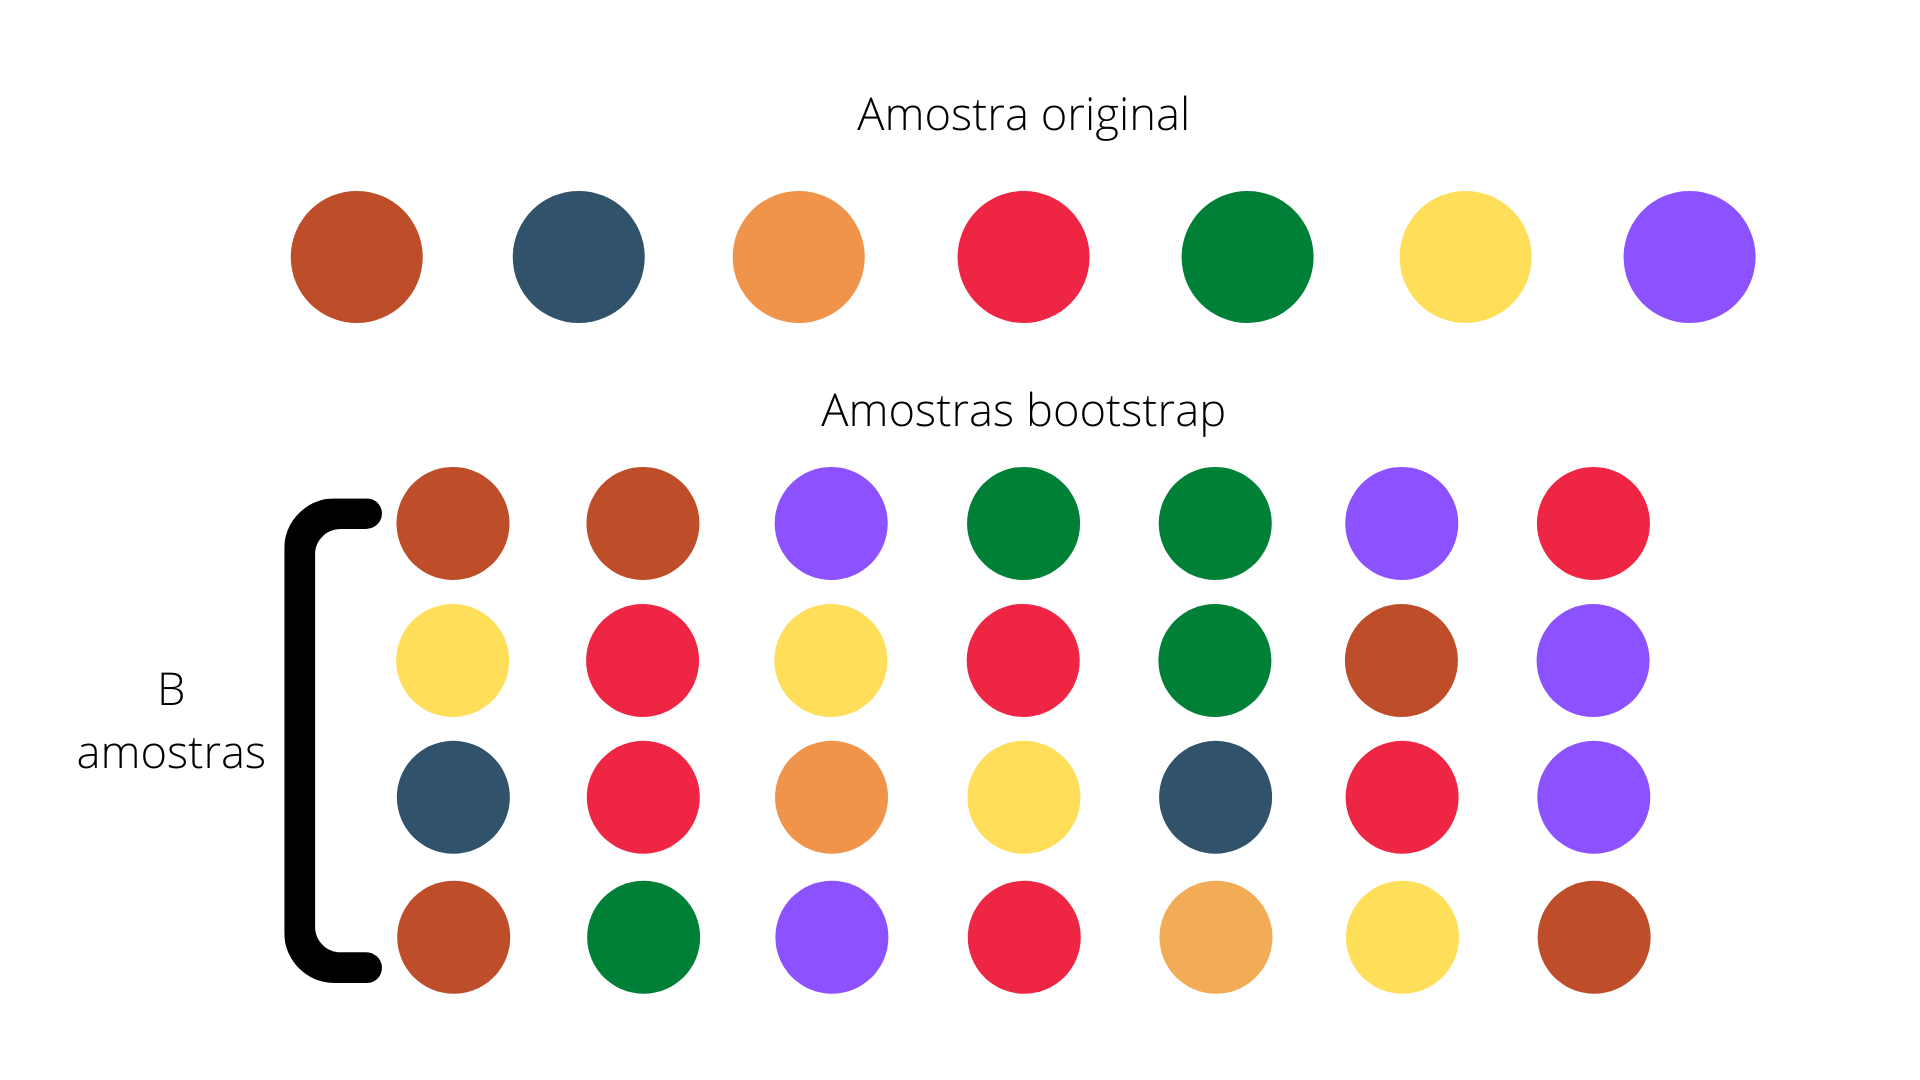
\includegraphics[width=\textwidth]{bootstrap.png}
    \end{figure}
    
\end{frame}

\begin{frame}{Estimador Monte Carlo}

    Para cada amostra, avaliamos $R^{(i)} = R(\boldsymbol{x}^{(i)},
\hat{F})$ e obtemos 
$$\{R^{(1)}, \dots, R^{(B)}\}.$$ 
Assim, teremos que 
$$
\frac{1}{B}\sum_{i=1}^B R^{(i)} \overset{P}{\to} \ev_{\hat{F}}[R], 
$$
pela Lei Forte dos Grandes Números. 

\bigskip\pause

No caso do erro padrão, 
$$
\hat{\sigma}_B = \left(\frac{1}{B-1}\sum_{i=1}^B (\hat{\theta}(\boldsymbol{x}^{(i)}) - \hat{\theta}^B)^2\right)^{1/2} \to \hat{\sigma}_{\hat{F}}.
$$

\end{frame}

\begin{frame}{Por que tamanho n?}

    Temos que $R(\boldsymbol{X}, F)$ depende de $n$ através de
    $\boldsymbol{X}$. A distribuição do estimador muda com $n$. Isso é fácil
    de ver quando $\hat{\theta}(\boldsymbol{x})$ é consistente. A demonstração
    clássica de Monte Carlo supõe que as variáveis são identicamente
    distribuídas.

    \bigskip\pause 

    \cite[]{bickel1981some} apresenta o seguinte teorema:

    \begin{figure}
        \centering
        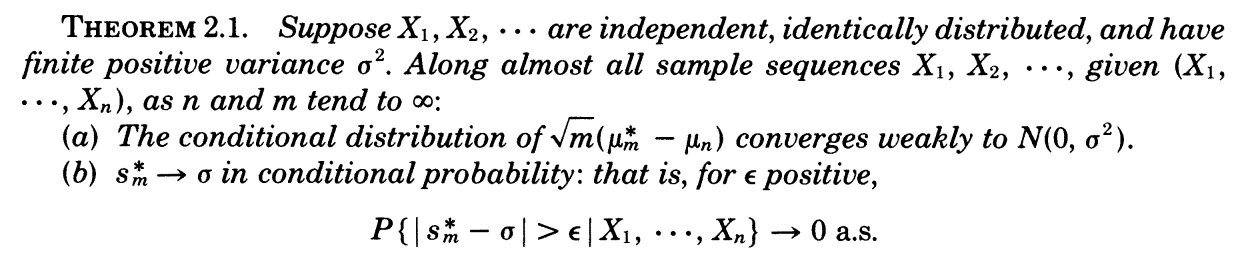
\includegraphics[width=\textwidth]{theorem-bickel}
    \end{figure}

\end{frame}

\begin{frame}{Bootstrap parametric}

    Se {\bf acreditamos} que $F$ vem de uma família, podemos usar seu
    Estimador de Máxima Verossimilhança para realizar o
    processo de re-amostragem.
    
\end{frame}

\begin{frame}{Jackknife}

    \begin{itemize}
        \item Método anterior ao bootstrap para estimar viés e variância de estimadores;
        
        \bigskip

        \item A ideia básica é deixar uma amostra de fora para cada
        re-amostragem e fazer o processo de estimar em cada amostra:
        $$
        \boldsymbol{x}_{(i)} = (x_1, x_2, \dots, x_{i-1}, x_{i+1}, \dots, x_n).
        $$
        
        \bigskip 

        \item O estimador de Jackknife para $\sigma_F$ é 
        $$
        \hat{\sigma}_J = \sqrt{\frac{n-1}{n}\sum_{i=1}^n (\hat{\theta}(\boldsymbol{x}_{(i)}) - \hat{\theta}^J)^2}.
        $$
    \end{itemize}
    
\end{frame}

%---------------------------------------------------

\begin{frame}[t, allowframebreaks]
  \frametitle{Referências}
  \bibliographystyle{apalike}
  \bibliography{stat_comp}
 \end{frame}

\end{document}